% Chapter 1

\chapter{Cost-Effectiveness Analysis Methodology} % Main chapter title

\label{sec:methodology} % For referencing the chapter elsewhere, use \ref{Chapter1} 

\section{Calibration}
Before starting the base analysis, we calibrate the transition matrices in the natural history by slightly modifying the original probabilities so that the output of our model (e.g. incidence, mortality, …) fits an observed value based on evidence. These calibrated probabilities can then be used by the rest of the strategies in the base analysis. See Calibration Workflow for more details.

\begin{figure}[h]
	\centering
	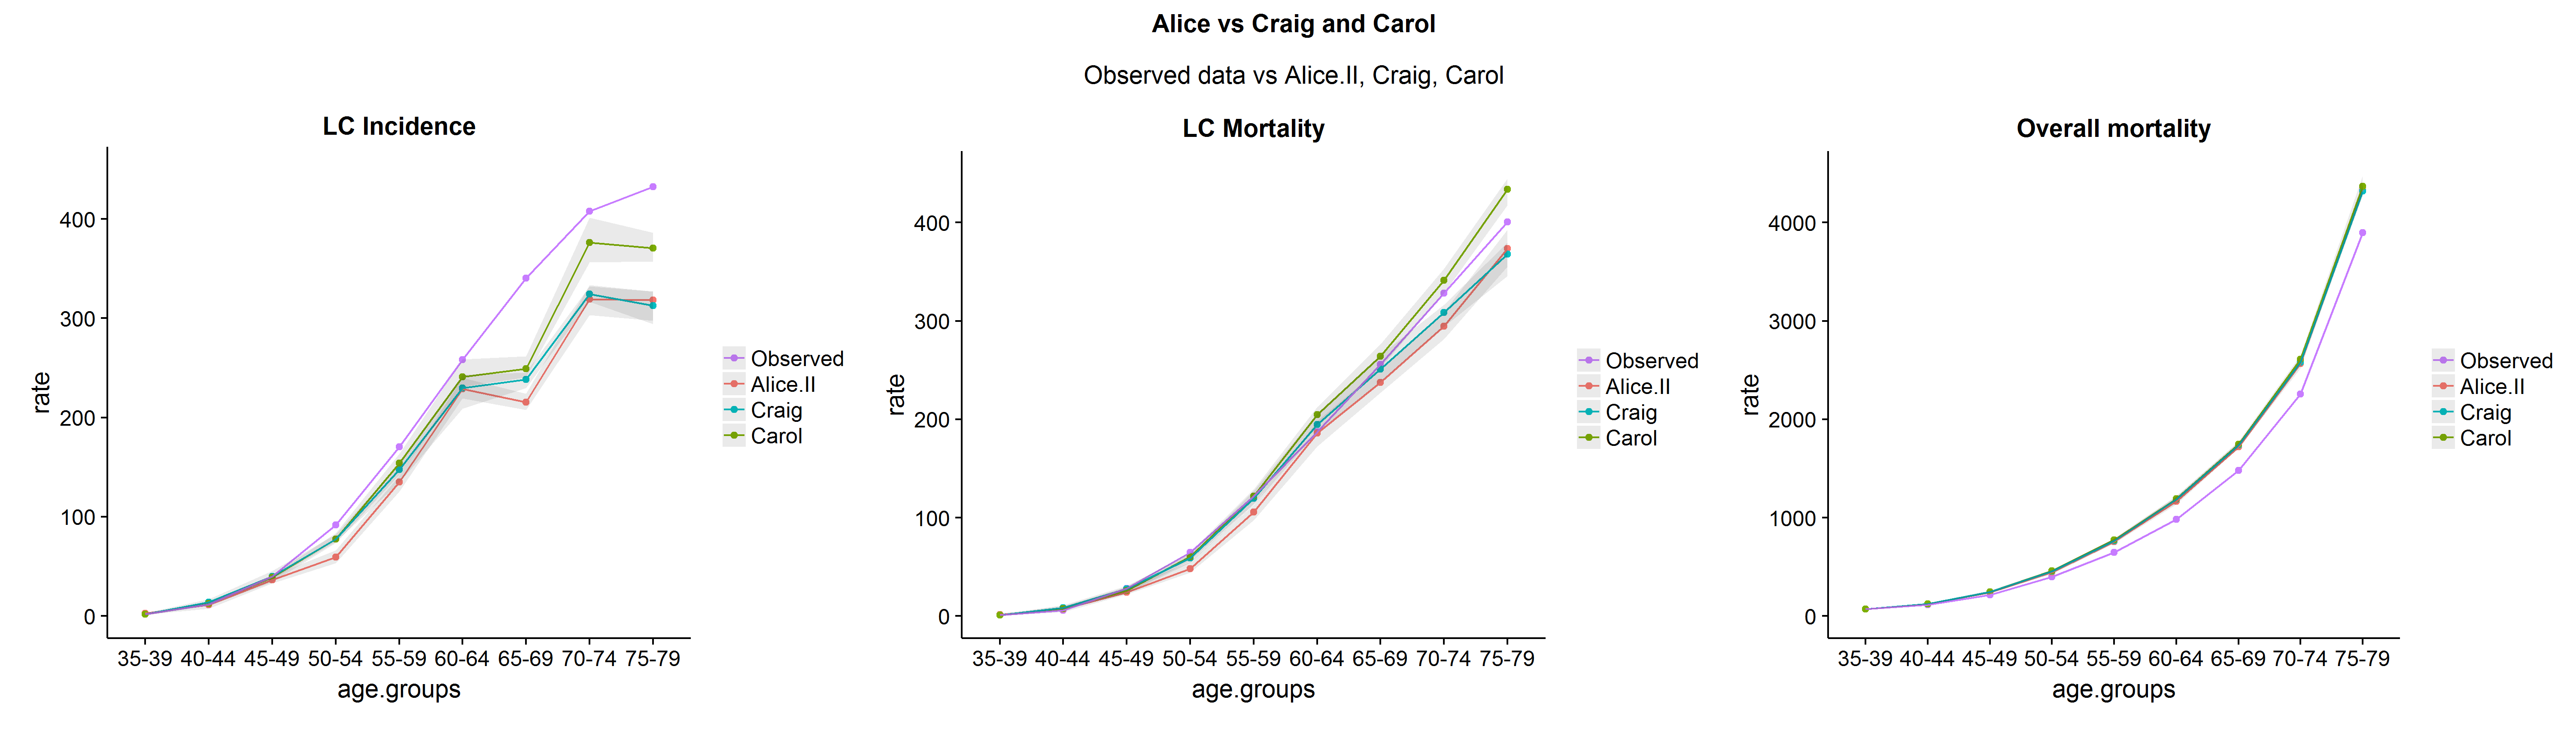
\includegraphics[width=\textwidth]{figures/lung_calibration_curves}
	\decoRule
	\caption[Calibration curve examples]{Example of three calibration curves for incidence, lung cancer mortality and mortality from other causes, along with the expected outcome.}
	\label{fig:lung_calibration_curves}
\end{figure}

\section{Base analysis}
Each strategy is plotted in the Cost and Effectiveness axes and the efficiency curve shows the strategies that are cost-effective, the rest are dominated by them and they are not considered cost-effective.

\begin{figure}[h]
	\centering
	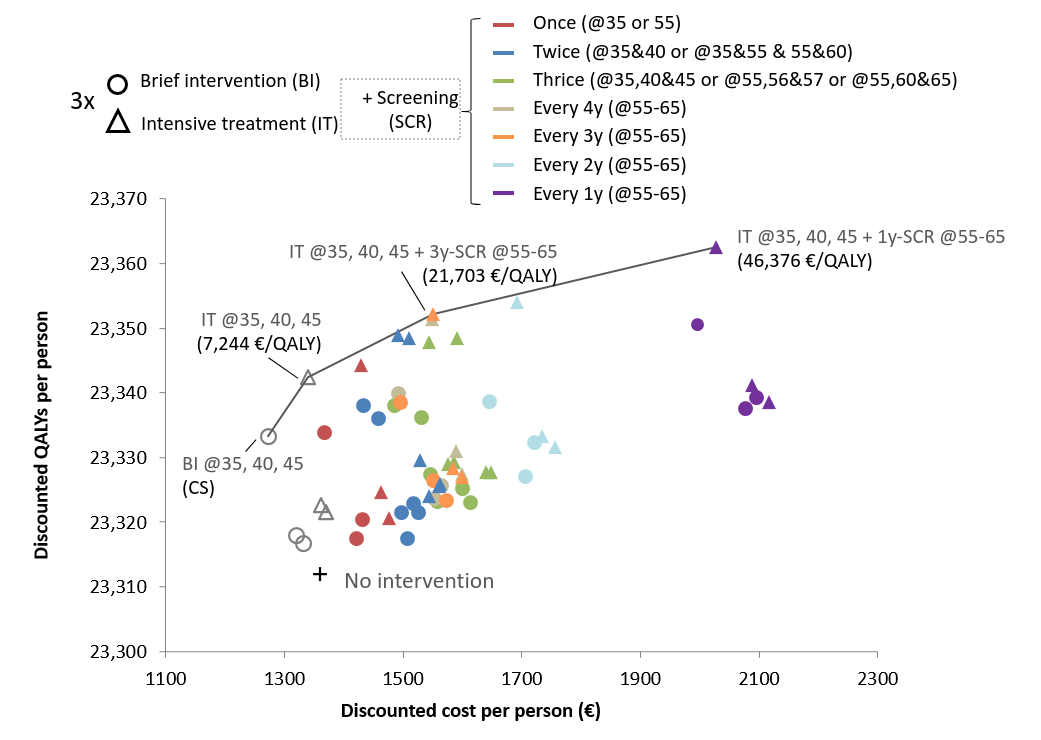
\includegraphics[width=\textwidth]{figures/lung_efficiency_curve}
	\decoRule
	\caption[Efficiency curve example]{Example of an efficiency curve showing the cost (€) and effectiveness (QALYs) of each of the simulated strategies. The strategies on the curve represent the cost-effective strategies, those below it are not usually considered since they are always dominated by one of those in the curve.}
	\label{fig:lung_efficiency_curve}
\end{figure}

We can compare each strategy in relation to another calculating the Incremental Cost-Effectiveness Ratio as:

$$
ICER=\frac{\Delta C}{\Delta E} = \frac{C_2-C_1}{E_2-E_1}
$$

If the ICER is below the Willingness-To-Pay (WTP) threshold (i.e. the maximum amount of money a country/region is willing to pay per additional QALY) the second strategy is more cost-effective than the first. If the ICER is greater than the WTP the strategy’s benefits are not considered cost-effective (i.e. the increased health benefit does not justify the increment of cost). Negative ICERs imply that one strategy dominates the other one.

\section{Sensitivity analysis}
Once the base analysis is performed we evaluate the uncertainty of the used parameters to check the robustness of the results. We modify the values of the parameters of interest to see how they affect the output of the model.

\subsection{Deterministic Sensitivity Analysis (DSA)}
A sweep is performed over a range (e.g. +-15\% of the base value) for the parameters of interest, to see how the ICER changes and whether the cost-effectiveness decision is different.

\begin{figure}[h]
	\centering
	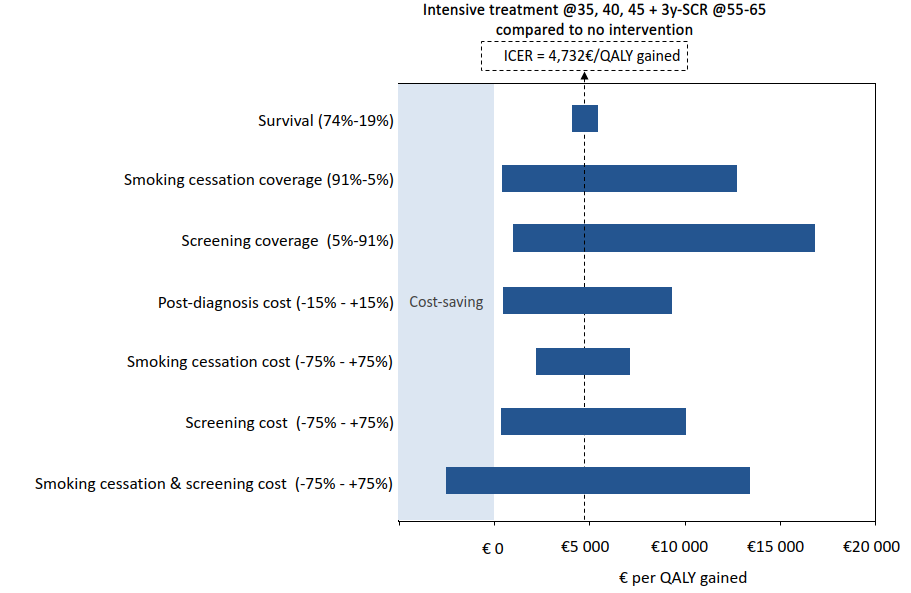
\includegraphics[width=\textwidth]{figures/lung_tornado}
	\decoRule
	\caption[Tornado diagram example]{Example of a tornado diagram showing the impact on the ICER between two particular strategies when changing one single parameter over a predefined range.}
	\label{fig:lung_tornado}
\end{figure}

\subsection{Probabilistic Sensitivity Analysis (PSA)}
Each parameter of interest is modeled as a probabilistic distribution (e.g. Beta for probabilities, Gamma/Lognormal for costs, ...) with the base value as the mean and a standard deviation dependent on the amount of uncertainty. We sample from these distributions (univariate or multivariate) to run a number of random simulations to check the percentage of simulations that show a cost-effective result (i.e. the percentage of simulations below the line ICER=WTP, see figure \ref{fig:endometrium_psa_scatterplot}).

\begin{figure}[h]
	\centering
	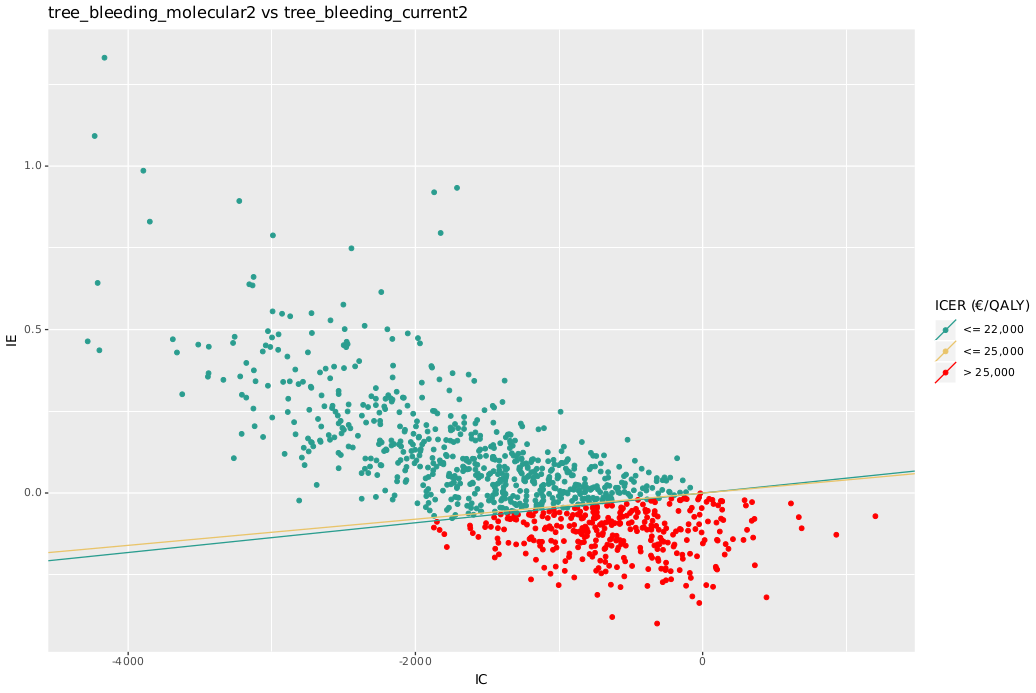
\includegraphics[width=\textwidth]{figures/endometrium_psa_scatterplot}
	\decoRule
	\caption[PSA scatterplot example]{Example of a scatterplot of a PSA, showing results from 1,000 random iterations and how they relate to the cost-effectiveness threshold (WTP). Green and red points represent cost-effective and non-cost-effective simulations respectively.}
	\label{fig:endometrium_psa_scatterplot}
\end{figure}